\section{Introduction}
\label{sec:introduction}

The pressing need for higher performance and efficiency pushes designers toward specialization -- navigating the efficiency / flexibility trade-off as visualized in \figref{fig:tradeOffArch}. Custom hardware (HW) implemented in an ASIC offers the highest efficiency and is combined the software cores to create application-specific platforms. However, (super-) specialization for each application individually is not a sustainable due to extremely high Non-Recurring Engineering (NRE) costs, limited deployment volumes and time to market pressure. Fully programmable but less specialized platforms (e.g. CPUs,  DSPs, GPUs) can be deployed much more widely to recover the NRE, but are magnitudes slower and less efficient. Domain-specific platforms can bridge the efficiency/flexibility gap, aiming at near ASIC performance and efficiency with sufficient flexibility to support applications within a domain (without necessarily being Turing complete). They dramatically increase the deployment potential making it much easier to recover the NRE. \newtext{However, this requires to broaden specialization from a narrow application focus to a more general domain specialization.} To enable scalable domain-specific computing, domain-aware innovations in design methodologies, tools, and architectures are needed. 


\begin{figure}
	%\vspace{-4pt}
	\centering
	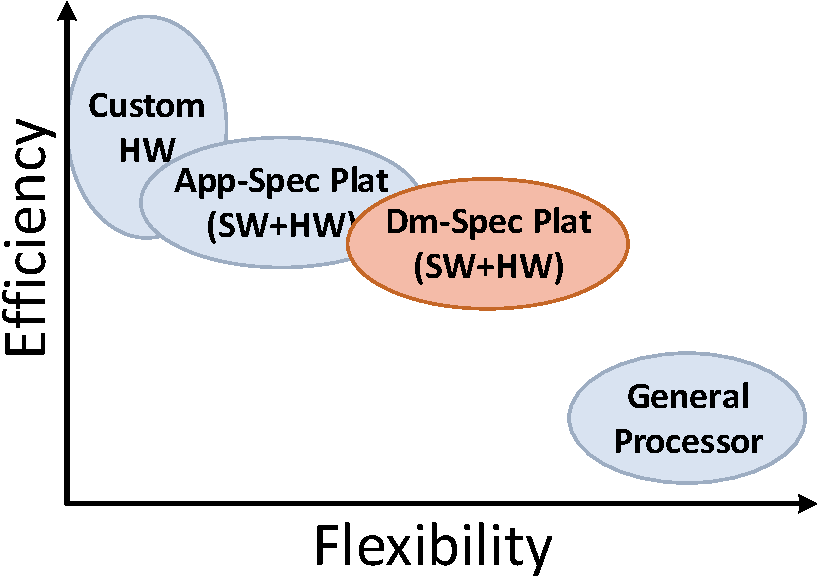
\includegraphics[width=.6\linewidth]{fig/pTradeOff.pdf}
	%\vspace{-6pt}
	\caption{Flexibility / Efficiency Trade-Off}
	\label{fig:tradeOffArch}
	%\vspace{-4pt}
\end{figure}


%\begin{wrapfigure}{l}{0.5\linewidth}
%	%\vspace{-6pt}
%	\begin{center}
%		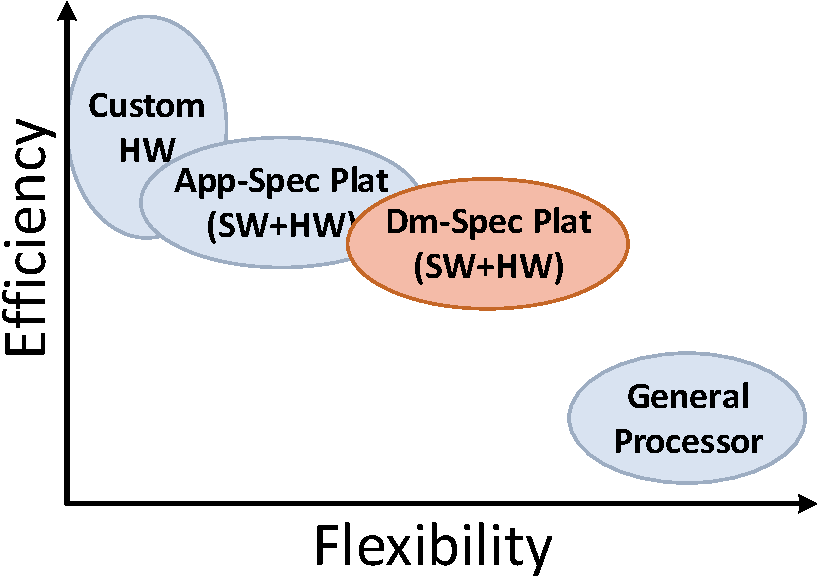
\includegraphics[width=\linewidth]{fig/pTradeOff.pdf}
%	\end{center}
%	%\vspace{-10pt}
%	\caption{Flexibility / Efficiency Trade-Off}
%	\label{fig:tradeOffArch}
%	\vspace{-4pt}
%\end{wrapfigure}

%\begin{figure}[t]
%    \centering
%    \subfloat[Flexibility / Efficiency]{
%       	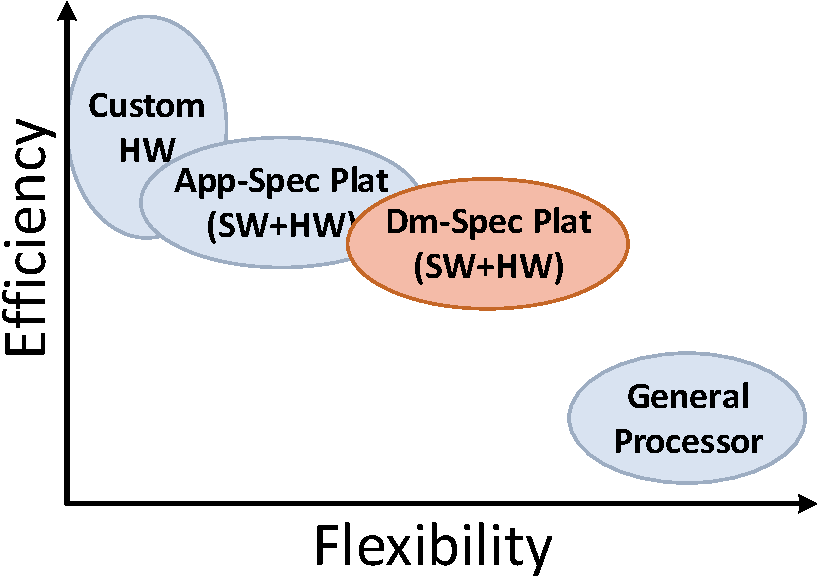
\includegraphics[width=.48\linewidth]{fig/pTradeOff.pdf}
%       	\label{fig:tradeOffArch}}
%    \hfill
%    \subfloat[Exploration / performance]{
%       	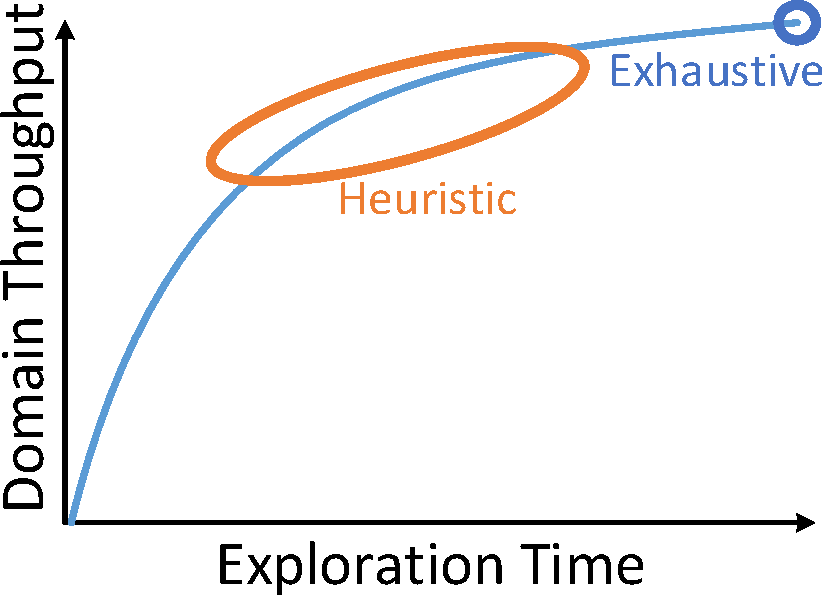
\includegraphics[width=.48\linewidth]{fig/pTradeOffAlg.pdf}
%       	\label{fig:tradeOffAlg}}
%		\vspace{-10pt}
%	\caption{Trade-Off for Platform and DSE}
%    \label{fig:trade-off}
%	\vspace{-10pt}
%\end{figure}

\begin{figure}[b]
		%\vspace{-20pt}
    \centering
        \subfloat[App-Specific Platform]{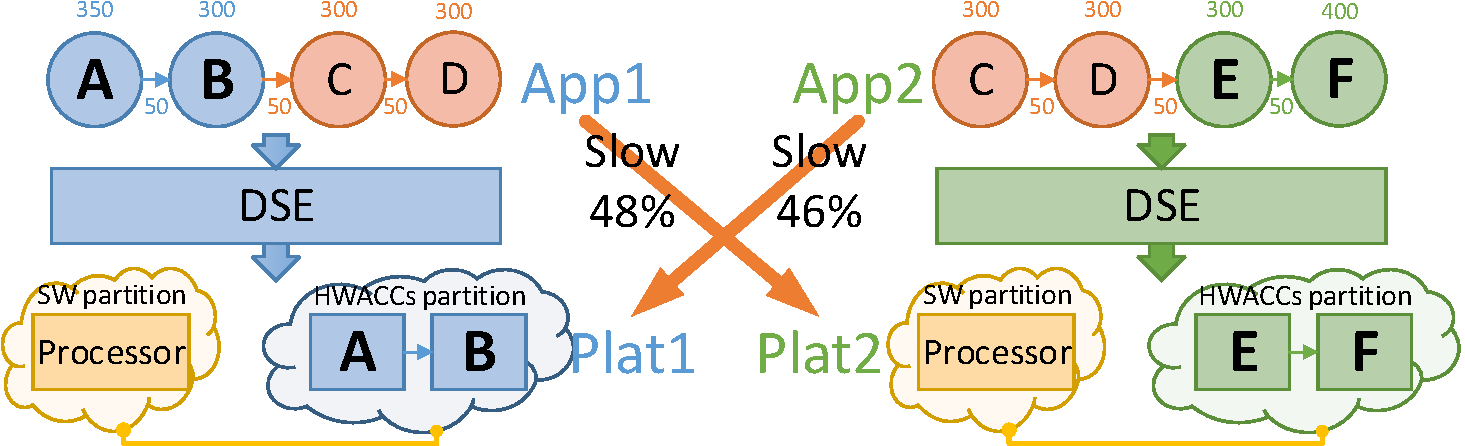
\includegraphics[width=.80\linewidth]{fig/pPlatApp.pdf}\label{fig:platApp}}
        \\ \vspace{-6pt}
        \subfloat[Domain-Specific Platform]{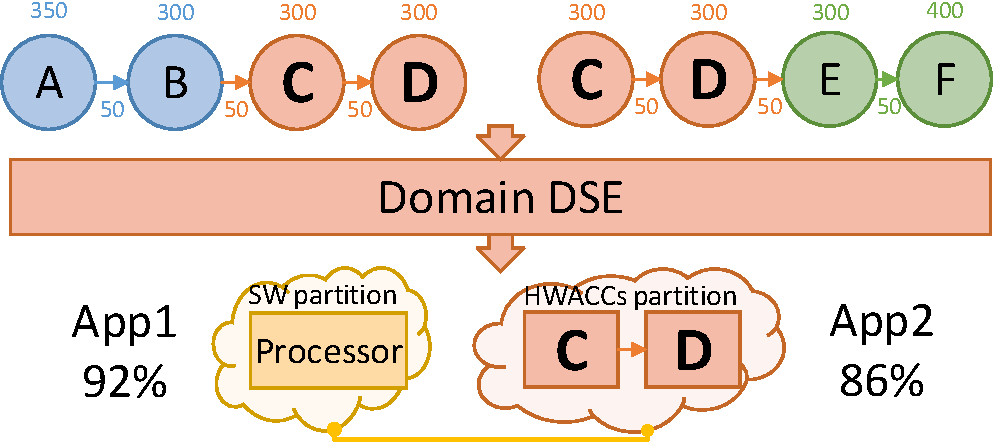
\includegraphics[width=.5\linewidth]{fig/pPlatDS.pdf}\label{fig:platDS}}
		%\vspace{-10pt}
    \caption{Domain Platform: Penalty of Application Scope}
    \label{fig:example}
\end{figure}


When moving to domain-platforms, few large monolithic accelerators make way for many smaller, composable accelerators. They offer configurable acceleration for selected compute-intensive kernels while running the remaining application in SW. Early domain-specific platforms include ACC-rich MPSoC~\cite{cong2014accelerator} or the Function-Level Processor~\cite{tabkhi2016function}. Domain-specific platforms aim at more specialization than typically considered in the platform-based design process, and target hardened implementations as opposed to reconfigurable computing  \cite{wildermann2011operational} paradigms.

%\figref{fig:tradeOffAlg} plots a domain DSE trade-off between exploration time and achievable domain throughput which is the result of identified domain function kernels for hardware acceleration. An exhaustive DSE throughout all possible design options (HW/SW choices over entire domain) can achieve the optimal domain throughput in the cost of excessive exploration time. Heuristic domain DSE algorithms are required that can offer near optimal accuracy with much shorter exploration time (traversing heuristic curve) to guide platform architects for finding the right balance and  HW/SW combinations for a domain.

Designing domain-specific platforms poses new challenges. 
While mapping multiple applications on an existing platform already received significant attention   \cite{kuang2005partitioning,wu2006low,abdeen2014multi,tang2015hardware}, 
designing domain platforms is less studied. 
Current DSE approaches primarily focus on a single application (one task graph) in isolation and do not address the domain optimization opportunities. 
The penalty of the narrow application focus is illustrated in \figref{fig:platApp}. Two platforms are each customized for an individual application, one accelerating $A$, $B$ and the other $E$, $F$. Executing each app on the other's platform results in low performance (48\%, 46\%).  Broadening the scope and considering both applications has tremendous benefits. The domain platform in \figref{fig:platDS} accelerates $C$, $D$ common to both applications. Now, both applications benefit from customization and execute at performance close to the own dedicated platform (92\%, 86\%). In order to explore the benefits of domain-specific platforms,  novel domain DSE tools and methodologies are needed that can identify functional and structural similarities across domain applications, utilize them for domain specialization, and rapidly evaluate the potential benefits for applications within a domain.

\newtext{This paper introduces a domain-specific design flow to aid HW/SW partitioning when designing a platform for a domain of applications. The key insight is to identify both behavioral (functional) and structural similarities across applications in a domain, and then evaluate benefits of the similarities in Domain DSE for HW/SW partitioning to optimize performance across all domain applications.}

\newtext{This paper introduces two novel Domain-Specific DSE approaches, Dynamic Score Selection (DSS) and GenetIc Domain Exploration (GIDE), to enable the domain-specific platform design. They focus on streaming applications (e.g. video analytics, software define radio) targeting platforms with many accelerators for high performance and power-efficient computing. Both, DSS and GIDE, broaden the scope of DSE from an individual application to a domain of applications. Instead of optimizing a platform for a single application, all domain applications are accelerated on the same domain platform.}

\newtext{DSS is our initial approach using a greedy algorithm. It introduces a Domain Score (DS) to rapidly estimate the change in benefits for the whole domain when changing HW/SW allocation. As a more comprehensive approach, we introduce} \ga \newtext{which uses utilizes high-level analytic models to improve evaluation accuracy (over DS).    
In addition,} \ga speeds up traversing the enormous design space using guided local search with a hybrid evaluation combining DS and Analytic Evaluation (AE). \newtext{Both approaches are evaluated in detail to highlight their characteristics and benefits. Their trade-off in exploration speed and accuracy is quantified. To the best of our knowledge, DSS and GIDE are the first greedy and genetic algorithms for domain design space exploration. 

In a nutshell, the contributions of this paper are:}

%This paper introduces GenetIc Domain Exploration (\ga), a novel Domain-Specific DSE enabling the domain-specific platform design process.
%\ga focuses on streaming applications (e.g. video analytics and software define radio) targeting platforms with many accelerators. \ga broadens the scope of Genetic Algorithms (GA) from an individual to a domain of applications. It defines assessing the benefit of a domain platform for its applications as the average throughput improvement over all applications. To speed up performance analysis in the evaluation, \ga utilizes high level analytical models. \ga speeds up traversing the enormous design space using guided local search with a hybrid evaluation combining Domain Score (DS) and  Analytic evaluation. In addition, its individual evaluation approaches are evaluated in detail to quantify their benefits in speed and accuracy. To the best of our knowledge, \ga is the first genetic algorithm for domain design space exploration. In a nutshell, the contributions of this paper are:

\begin{enumerate}
    \item Defining quantifiable domain features to express the similarities among applications.
    \item Providing a domain analyzer to extract domain features from applications.
    \item Introducing Domain Score (DS) to compare relative benefit of a platform in domain level.
    \item Accelerating the evaluation of domain-platforms fitness for a group of applications through Analytic Evaluation (AE).
    \item Introducing the first greedy algorithm Dynamic Score Selection (DSS) using DS for rapid Domain-Specific Design Space Exploration (DS-DSE).
    \item Introducing the first genetic algorithm GenetIc Domain Exploration (GIDE) for DS-DSE. In \ga, accelerating the design space traversal through guided local search using a hybrid of DS and AE.
    \item Providing a methodology to evaluate platforms in context of domains.
    \item Exploring the speed versus accuracy trade-off for domain exploration.
\end{enumerate}

%One major contribution of this paper encoding domain platform options to GA chromosomes coupled with the guided local search to narrow down the domain design space. For the GA guided local search, this paper proposes two domain evaluation options: (1)  which offers faster evaluation, but lower accuracy. (2) Analytical which offers higher accuracy but slower evaluation. The GA algorithm is coupled with multiple variations of guided local search (DSS, analytical, or hybrid) to create a balance between domain exploration time and evaluation accuracy (which can lead to higher domain throughput). 
%JH comment: There is no clear contribution summary in Introduction.

The benefits of DSS and \ga are demonstrated using 40 applications from the video analytics domain based on OpenVX \cite{Intel, AMD}, as well as varying synthetic domains. \newtext{Results are compared against application-specific designs and domain optimal results (obtained through exhaustive search) wherever possible.}
\newtext{The DSS} and \ga generated platform achive significant performance improvement: 23.60\%-58.02\% and 48.09\%-74.85\% on average compared to application-specific platform designs.
\newtext{DSS achieves 93.65\% and 83.45\% of domain optimal throughput for OpenVX and synthetic domain, with $10^{17}$ times faster than exhaustive search. While GIDE reaches 99.87\% and 98.84\% of domain optimal throughput, with $10^{13}$ times faster exploration compared with exhaustive search.}
\newtext{GIDE achieves 10.65\% (OpenVX) and 19.81\% (synthetic) higher domain throughput improvement than DSS.}
With this, \ga enables rapid domain design space exploration producing high quality results.

%The benefits of \ga are demonstrated using 40 applications from the video analytics domain based on OpenVX \cite{Intel, AMD}, as well as varying synthetic domains. Results are compared against optimal results (obtained through exhaustive search) wherever possible, and an existing heuristic approach - Domain Score Selection (DSS)~\cite{zhang100ds}. \ga reaches 99.8\% and 97.6\% of domain optimal throughput for OpenVX and synthetic domains, with $10^{13}$ times faster exploration than exhaustive search. 
%Compared to the greedy DSS, \ga achieves 10.65\%  and 19.81\% higher domain throughput improvement for OpenVX and synthetic domains. With this, \ga enables rapid domain design space exploration producing high quality results.

\begin{figure}[h]
	\centering
	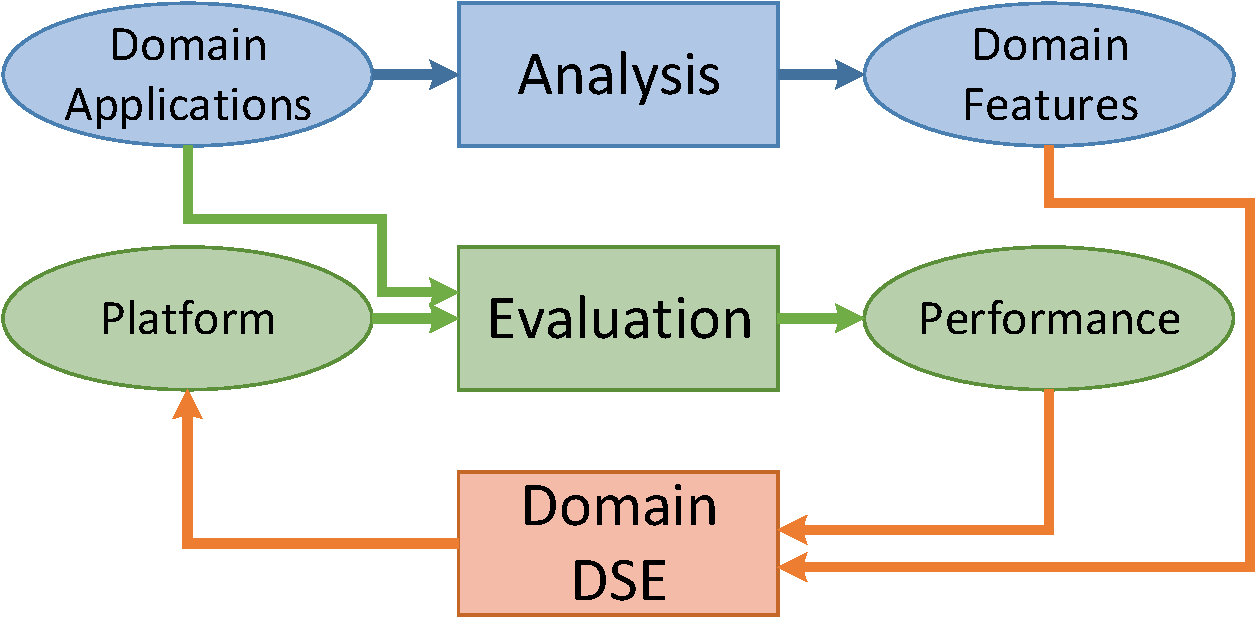
\includegraphics[width=.65\linewidth]{fig/Overview.pdf}
	\caption{Domain DSE Overview}
	\label{fig:overview}
\end{figure}

\figref{fig:overview} \newtext{describes the flow and challenges of Domain DSE. Domain features are need to be identified and extracted from domain applications. A methodology is necessary to evaluate the performance of domain platform. Domain-level DSE algorithms are needed to explore the large domain design space. This paper is organized as follows:} \secref{sec:related} summarizes the related work. \secref{sec:Domain} identifies domain features metrics and presents domain features analyzer. \secref{sec:EvaOp} introduces target domain platform and our proposed platform evaluation models. \secref{sec:DSE} defines domain DSE problem. \secref{sec:DSS} introduces the DSS algorithm for domain HW/SW partitioning. \secref{sec:GA} introduces \ga incrementally from genetic algorithm with random mutation to guided local search. \secref{sec:results}  evaluates and analyses DSS and \ga benefits providing detailed performance insights. 
%\secref{sec:generalization} summarizes all algorithms in DSE trade-off. 
Finally \secref{sec:conclusion} concludes this paper. 